\documentclass{standalone}
\usepackage{mintikz}

\begin{document}
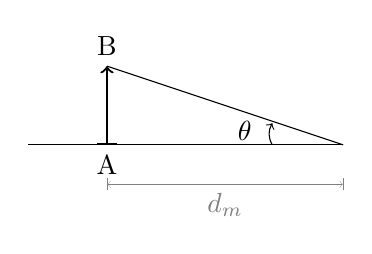
\begin{tikzpicture}[] 
    %\draw [ultra thin, gray!20] (-6,-6) grid[step=0.5] (6,6);
    %\draw [thin,gray!50] (-6,-6) grid[step=1] (6,6);
    \def \taillehaut{2}; %taille de la lentille
    \def \taillebas{2};%taille de la lentille
    \def \xA{-1};%position de l'objet
    \def \yB{1};%hauteur de l'objet
    \def \xAA {(\xA*\f)/(\xA+\f)};%position de l'image
    \def \yBB {(\xAA*\yB)/(\xA)};%hauteur de l'image
    \coordinate (O1) at (0,0);%centre optique de la première lentille
    \coordinate (A) at (\xA,0);%position de l'objet
    \coordinate (B) at (\xA,\yB);%sommet de l'objet
    \def \f{2};%focale de la première lentille
    \coordinate (F') at (\f,0);
    \coordinate (A') at ({\xAA},0);%position de l'objet
    \coordinate (B') at ({\xAA},{\yBB});%sommet de l'objet
    
    
    \draw[|->, thick]  (A)node[below]{A}--(B)node[above]{ B};
    \draw[thin](-2,0)--++(4,0);
    
    \draw[ultra thin,gray,|<->|](-1,-0.5)--(2,-0.5) node [midway, below]
        {$\text{d}_\text{m}$};
    
    \draw (B) -- (2,0);
    
    \draw[->] (1.1,0) to [bend left] (1.1,0.275) ;
     \node at (0.75,0.175) [] {$\theta$};
    \oeil[shift={(2.8,0)},rotate=180];

\end{tikzpicture}

\end{document}
